

\section{Introduction}
\index{Scenario Risk}
The scenario risk calculator is capable of computing losses and loss statistics from a single event for a collection of assets, given a set of \glspl{groundmotionfield}. The use of a set of \glspl{groundmotionfield} is recommended so that the aleatory variability (both inter- and intra-event) in the \gls{groundmotionpredictioneq} is modelled. The input \glspl{groundmotionfield} can be calculated with oq-hazardlib or by an external software; in either case they need to be stored in the OpenQuake engine database. With the use of the oq-hazardlib, these \glspl{groundmotionfield} can be calculated either with or without the spatial correlation of the ground motion residuals.

For each \gls{groundmotionfield}, the intensity measure level at a given site is combined with a \gls{vulnerability function}, from which a loss ratio is randomly sampled, for each \gls{asset} contained in the \gls{exposure model}. The loss ratios that are sampled for \glspl{asset} of a given \gls{taxonomy} classification at different locations can be considered to be either independent, fully correlated, or correlated with a specific correlation coefficient. Using these results, the mean and standard deviation of the loss ratios across all \glspl{groundmotionfield} can be calculated. Loss ratios are converted into \gls{groundupLosses} by multiplying by the cost (which can be the structural, non-structural or contents) of the \gls{asset} given in the exposure model. It is furthermore possible to sum the losses throughout the region and to compute the mean and standard deviation of the total loss. This process is common to any of the costs type (structural, non-structural or contents) or occupants.
Besides the \gls{groundupLosses}, it is also possible to calculate \gls{insuredLosses} (i.e. economic value that can be covered by the insurance industry according to a certain policy). To do so, both a \gls{deductible} and a \gls{limit} for each type of cost (structural, non-structural or contents) need to be defined. The methodologies employed to calculate the \gls{groundupLosses} and \gls{insuredLosses} are described below.

\section{Calculation Steps}

To compute the mean \gls{groundupLosses}:

\begin{enumerate}
\item For each \gls{groundmotionfield}, the intensity measure level at the location of the \gls{asset} is used to derive the mean loss ratio and associated coefficient of variation from the \gls{vulnerability function}. Since currently the \glspl{vulnerability function} are being defined in a discrete manner, it is quite probable that the intensity measure level provided by the \gls{groundmotionfield} is not contained in the \gls{vulnerability function}. In these cases, linear interpolation methods are being employed to derive the mean loss ratio at the intensity measure level of interest. 

\item The engine takes the \gls{vulnerability function} assigned to each \gls{asset} and checks if the coefficient of variation is zero. If so, the loss ratios are derived based on the mean loss ratio for each intensity measure level. Otherwise, if the uncertainty is defined, it is randomly sampled following the probabilistic distribution of the respective \gls{vulnerability function}, as described below:

\begin{equation}
\log{LR_n} = \mu + \epsilon\sigma
\end{equation}

Where $\mu$ and $\sigma$ stand for the mean and standard deviation of the logarithm of the loss ratios, respectively, and $\epsilon$ is a term that has a standard normal distribution with a zero mean and a standard deviation of one.  

The method used to sample epsilon depends on whether the correlation between the vulnerability uncertainty of \glspl{asset} of a given \gls{taxonomy} is to be considered or not:

\begin{itemize}

\item Perfectly correlated: the term $\epsilon$ is randomly sampled once for the first \gls{asset} and this result is used to derive the loss ratio for all the \glspl{asset} of the same \gls{taxonomy}. 

\item Correlated: the term $\epsilon$ is randomly sampled for each \gls{asset} considering the specified correlation coefficient between \glspl{asset}. 

\item Uncorrelated: the term $\epsilon$ is always randomly sampled for each \gls{asset} and therefore the correlation between the vulnerability of the \glspl{asset} is ignored.

\end{itemize}

\item The mean loss ratio for each \gls{asset} across all possible simulations of the scenario event can be calculated through the formula:

\begin{equation}
LR=\frac{\sum^m_{n=1}LR_n|IML}{m}
\end{equation}

Where $m$ stands for the number of ground motion fields simulated.

\item The mean loss can then be derived by multiplying the mean loss ratio by the value of the \gls{asset} contained in the \gls{exposure model} file.

\end{enumerate}

To compute the standard deviation of the ground-up losses:

\begin{enumerate}

\item In order to compute the uncertainty, the engine takes the set of loss ratios for each \gls{asset}, and computes the associated standard deviation using the classical formula:

\begin{equation}
SD[LR]=\sqrt{  \frac{1}{m}\sum_{n=1}^m{(LR_n-E[LR])^2} }
\end{equation}

Where $E[LR]$ stands for the mean loss ratio computed previously.

\item The standard deviation of the absolute loss can finally be computed by multiplying the standard deviation of the loss ratio by the value of the respective \gls{asset}.

\end{enumerate}

To compute the \gls{insuredLosses}:
The calculation of the insured losses is valid for the structural, non-structural and contents costs. When the computation of the insured losses is triggered, the ground-up losses from each asset, at each \gls{groundmotionfield} are modified in the following manner:

\begin{enumerate}

\item If the limit has been defined in a relative way, this fraction is first multiplied by the respective total cost, in order to obtain the absolute value. If the ground-up loss is above the absolute limit, the resulting loss is reduced to this threshold.

\item Then, the absolute deductible is taken directly from the exposure model, or calculated by multiplying the associated fraction by the respective total cost. Once the absolute deductible is obtained, the ground-up loss is further reduced by this amount. If the deductible is above the ground-up loss, then the insured loss is null.

This process is clarified in Figure \ref{fig:insuredLosses}.

\begin{figure}[ht]
\centering
\includegraphics[width=14cm,height=7cm]{./figures/risk/insuredLosses.eps}
\caption{Representation of the process to estimate the insured losses.}
\label{fig:insuredLosses}
\end{figure} 

In Case A, the ground-up loss does not exceed the deductible, which leads to an insured loss equal to zero. In Case B, the ground-up loss is above the deductible, but does not reach the limit. Hence, the resulting insured loss if equal to the ground-up loss minus the deductible. Finally, in Case C the ground up loss is greater than the limit. Thus, this loss is firstly reduced to the value of the limit, and then  the deductible is subtracted. In other words, the portion of the ground-up losses that are insured, is the fraction located between the deductible and the limit thresholds.   

\item The calculation of the mean and standard deviation of the insured losses follows the same approach described previously for the ground-up losses.

\end{enumerate}

\section{Calculator Output}
The output of the Scenario Risk Calculator currently comprises ground-up and insured loss statistics (mean total loss and standard deviation of total loss) and ground-up and insured loss maps. Loss maps are comprised by a set of loss nodes, which are associated with a pair of coordinates. For each node, one or more loss values might exist, due to the fact that several different \glspl{asset} can be located at the same location.  Figure \ref{fig:detlosses} presents an example of a loss map containing the expected economic losses for residental buildings located in Nepal, considering a rupture of magnitude 7.0Mw in the central part of the country.

\begin{figure}[ht]
\centering
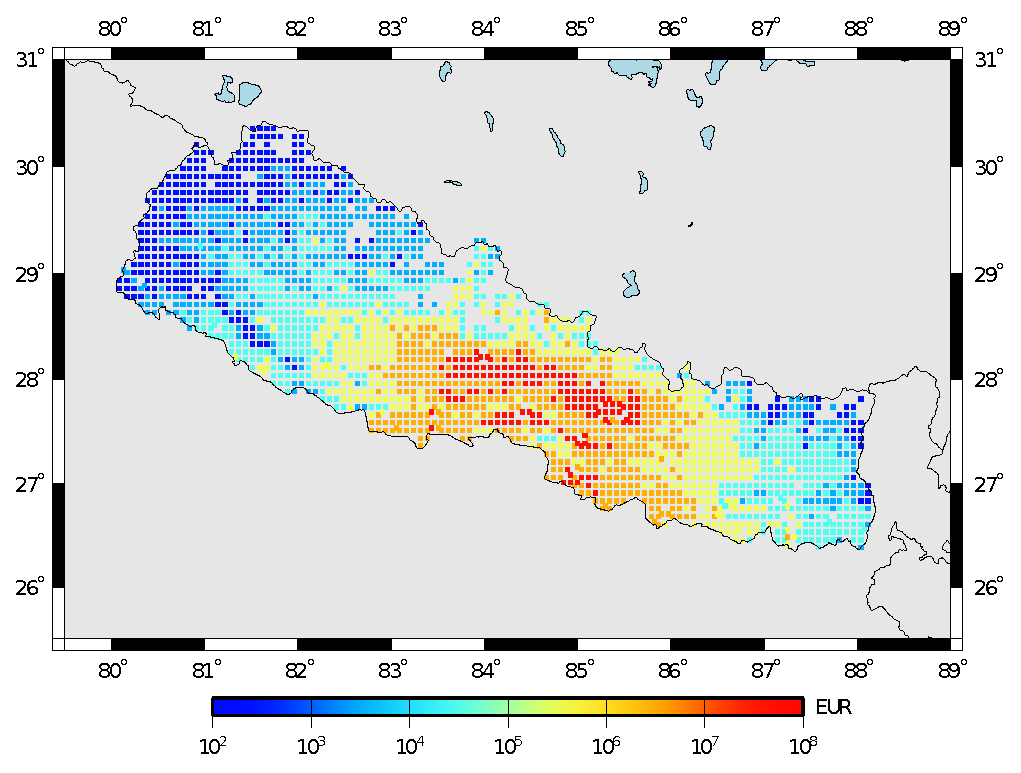
\includegraphics[width=12cm,height=8cm]{./figures/risk/LossmapDet.eps}
\caption{Loss map with the distribution of mean economic losses for residential buildings in Nepal.}
\label{fig:detlosses}
\end{figure} 